\section{User Authentication Methodologies}
\label{s:authAuth}

In the context of users, \gls{authentication} is proving a
the system who you are; e.g., a daily average of 217
million people authenticate themselves on Twitter by
logging in to their account \parencite[][Q4]{twitterUsage}.

In such a case, a user may provide their Twitter username
and password, known as \textbf{credentials}; i.e.,
\enquote{an agreed piece of information shared between the
  user and the system} \parencite{whatIsAuth}.

An authentication \textbf{factor} is considered to be a
\enquote{specific category of credentials}
\parencite{whatIsAuth}.
By categorising credentials, we can understand the
requirements (e.g., hardware, software, cost, etc.) and
constraints (e.g., accessibility, security, etc.) of many
authentication schemes at once.

As such, factors save time and effort when determining the
viability of authentication schemes for a system.
For example, any scheme within the
\hyperref[p:knowledge]{knowledge factor} would not be
appropriate for a userbase with memory impairment.

Moreover, factors can be used in tandem to create a more
complex authentication process, as shown in
Figure~\ref{fig:github2fa}.
\cite{whatIsAuth} describes
\textbf{two-factor authentication} (2FA) as
\enquote{authentication mechanism based on two categories
  of credentials}, with additional factors generalised as
\textbf{multi-factor} (MFA).

\begin{figure}[h]
  \centering
  \begin{subfigure}{\subfigwidth}
    \centering
    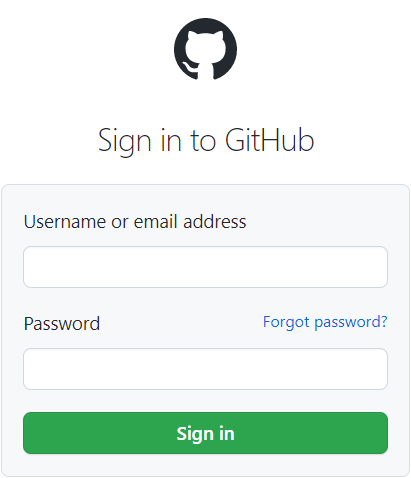
\includegraphics[width=0.75\linewidth]{04
      research/assets/github factor 1.png}
    \caption{First factor:
      \hyperref[ss:passwords]{password}}
  \end{subfigure}
  \begin{subfigure}{\subfigwidth}
    \centering
    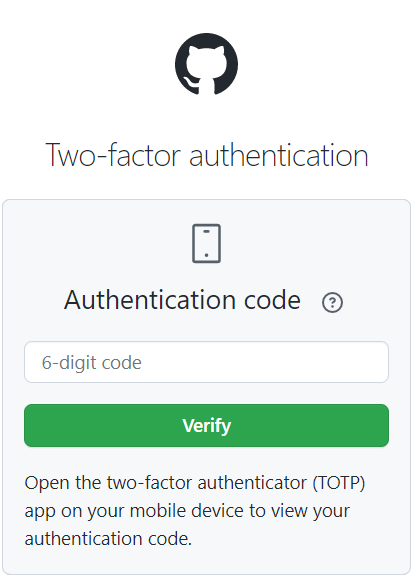
\includegraphics[width=0.75\linewidth]{04
      research/assets/github factor 2.png}
    \caption{Second factor: \hyperref[ss:otp]{OTP}}

  \end{subfigure}

  \caption{2FA with Github}
  \label{fig:github2fa}
\end{figure}

Described by \cite{surveyOnAuthFactors}, the three most
common authentication factors are: 

\begin{itemize} 

  \item \textbf{Knowledge} \label{p:knowledge} refers to
        \enquote{something that a user knows}, such as a PIN.
        The main aspect of security it holds is the secrecy of the
        data: only those who know can authenticate.

  \item \textbf{Possession} refers to \enquote{something
          that a user [physically] possesses}, such as an
        \hyperref[ss:otp]{OTP}.

  \item \textbf{Inherence} refers to \enquote{something
          that a user is}.
        This can be a physical characteristic, such as a
        fingerprint, or cognitive, which authenticates by reading
        an individuals thought processes.
\end{itemize}

\subsection{Passwords}
\label{ss:passwords}
Passwords are knowledge-based; a person memorises an
ordered sequence of data against which the authenticator
can check its own records to approve/deny the
authentication.

The forms of a password are many, however they are most
often typed: the classic example is a character string,
with  constraints on complexity and minimum length; a
Personal Identification Number (PIN) is another everyday
application in banking \parencite{whatIsAuth}; and less
common is a pattern-based password, as seen on Android lock
screens \parencite{androidLockScreen}.

\subsection{One-time Passwords (OTP)}
\label{ss:otp}

OTPs are passwords which can only be used once.
After being generated by the authenticator, they are sent
securely to the user to be entered and subsequently
verified \parencite{surveyOnAuthFactors}.

Any device with SMS capabilities can receive one-time
passwords; smartphones are also able to receive/generate
OTPs using dedicated apps like
\href{https://www.twilio.com/authy/features/totp}{Authy}
and \href{https://play.google.com/store/apps/details?
  id=com.google.android.apps.authenticator2}{Google}.
In this case, an OTP can be categorised as a knowledge
factor\parencite{surveyOnAuthFactors, evalOfAuthMethods}.
Alternatively, proprietary devices named \enquote{tokens}
can also generate OTPs, including RSA SecurID, USB tokens
such as Yubikey2, and RFID keys.
Figure~\ref{fig:otp} demonstrates both devices used to
receive one-time passwords.
\cite{evalOfAuthMethods} considers tokens
as a possession factor, whereas
\cite{surveyOnAuthFactors} considers them as
knowledge.

\begin{figure}[h]
  \centering
  \begin{subfigure}{\subfigwidth}
    \centering
    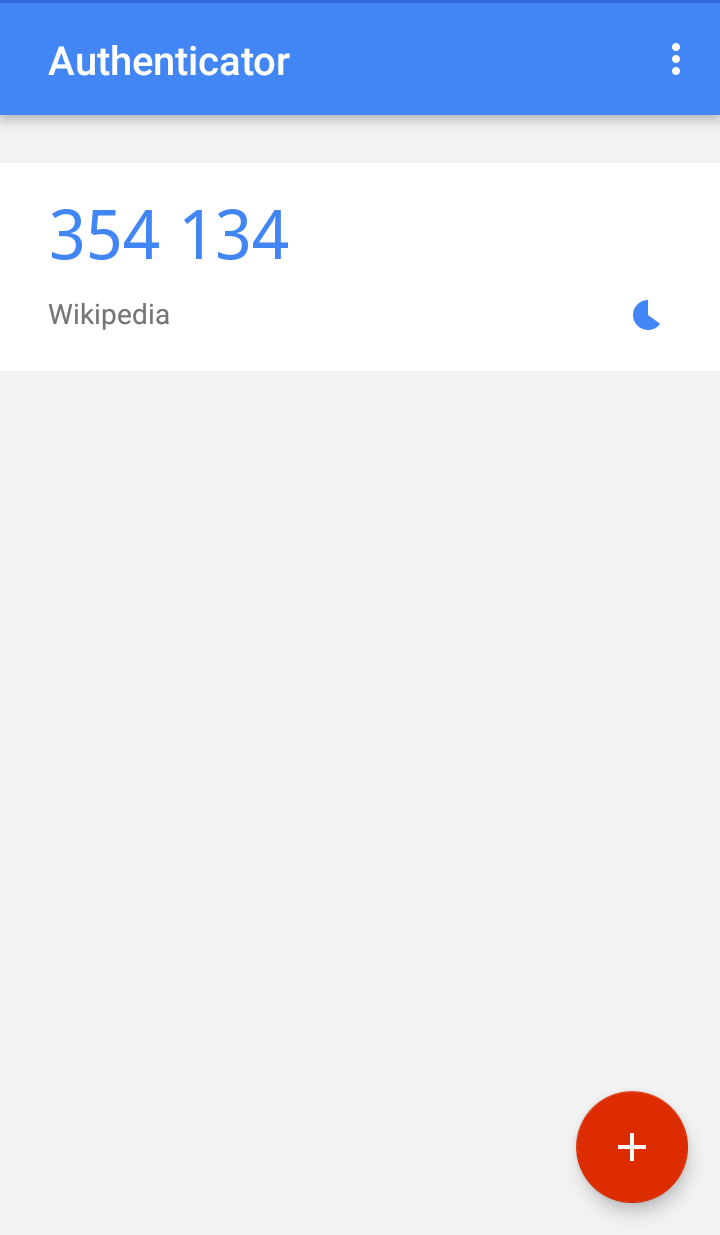
\includegraphics[width=0.6\linewidth]{04
      research/assets/google authenticator.png}
    \caption{Google Authentication}
    \parencite{img:googleAuth}
  \end{subfigure}
  \begin{subfigure}{\subfigwidth}
    \centering
    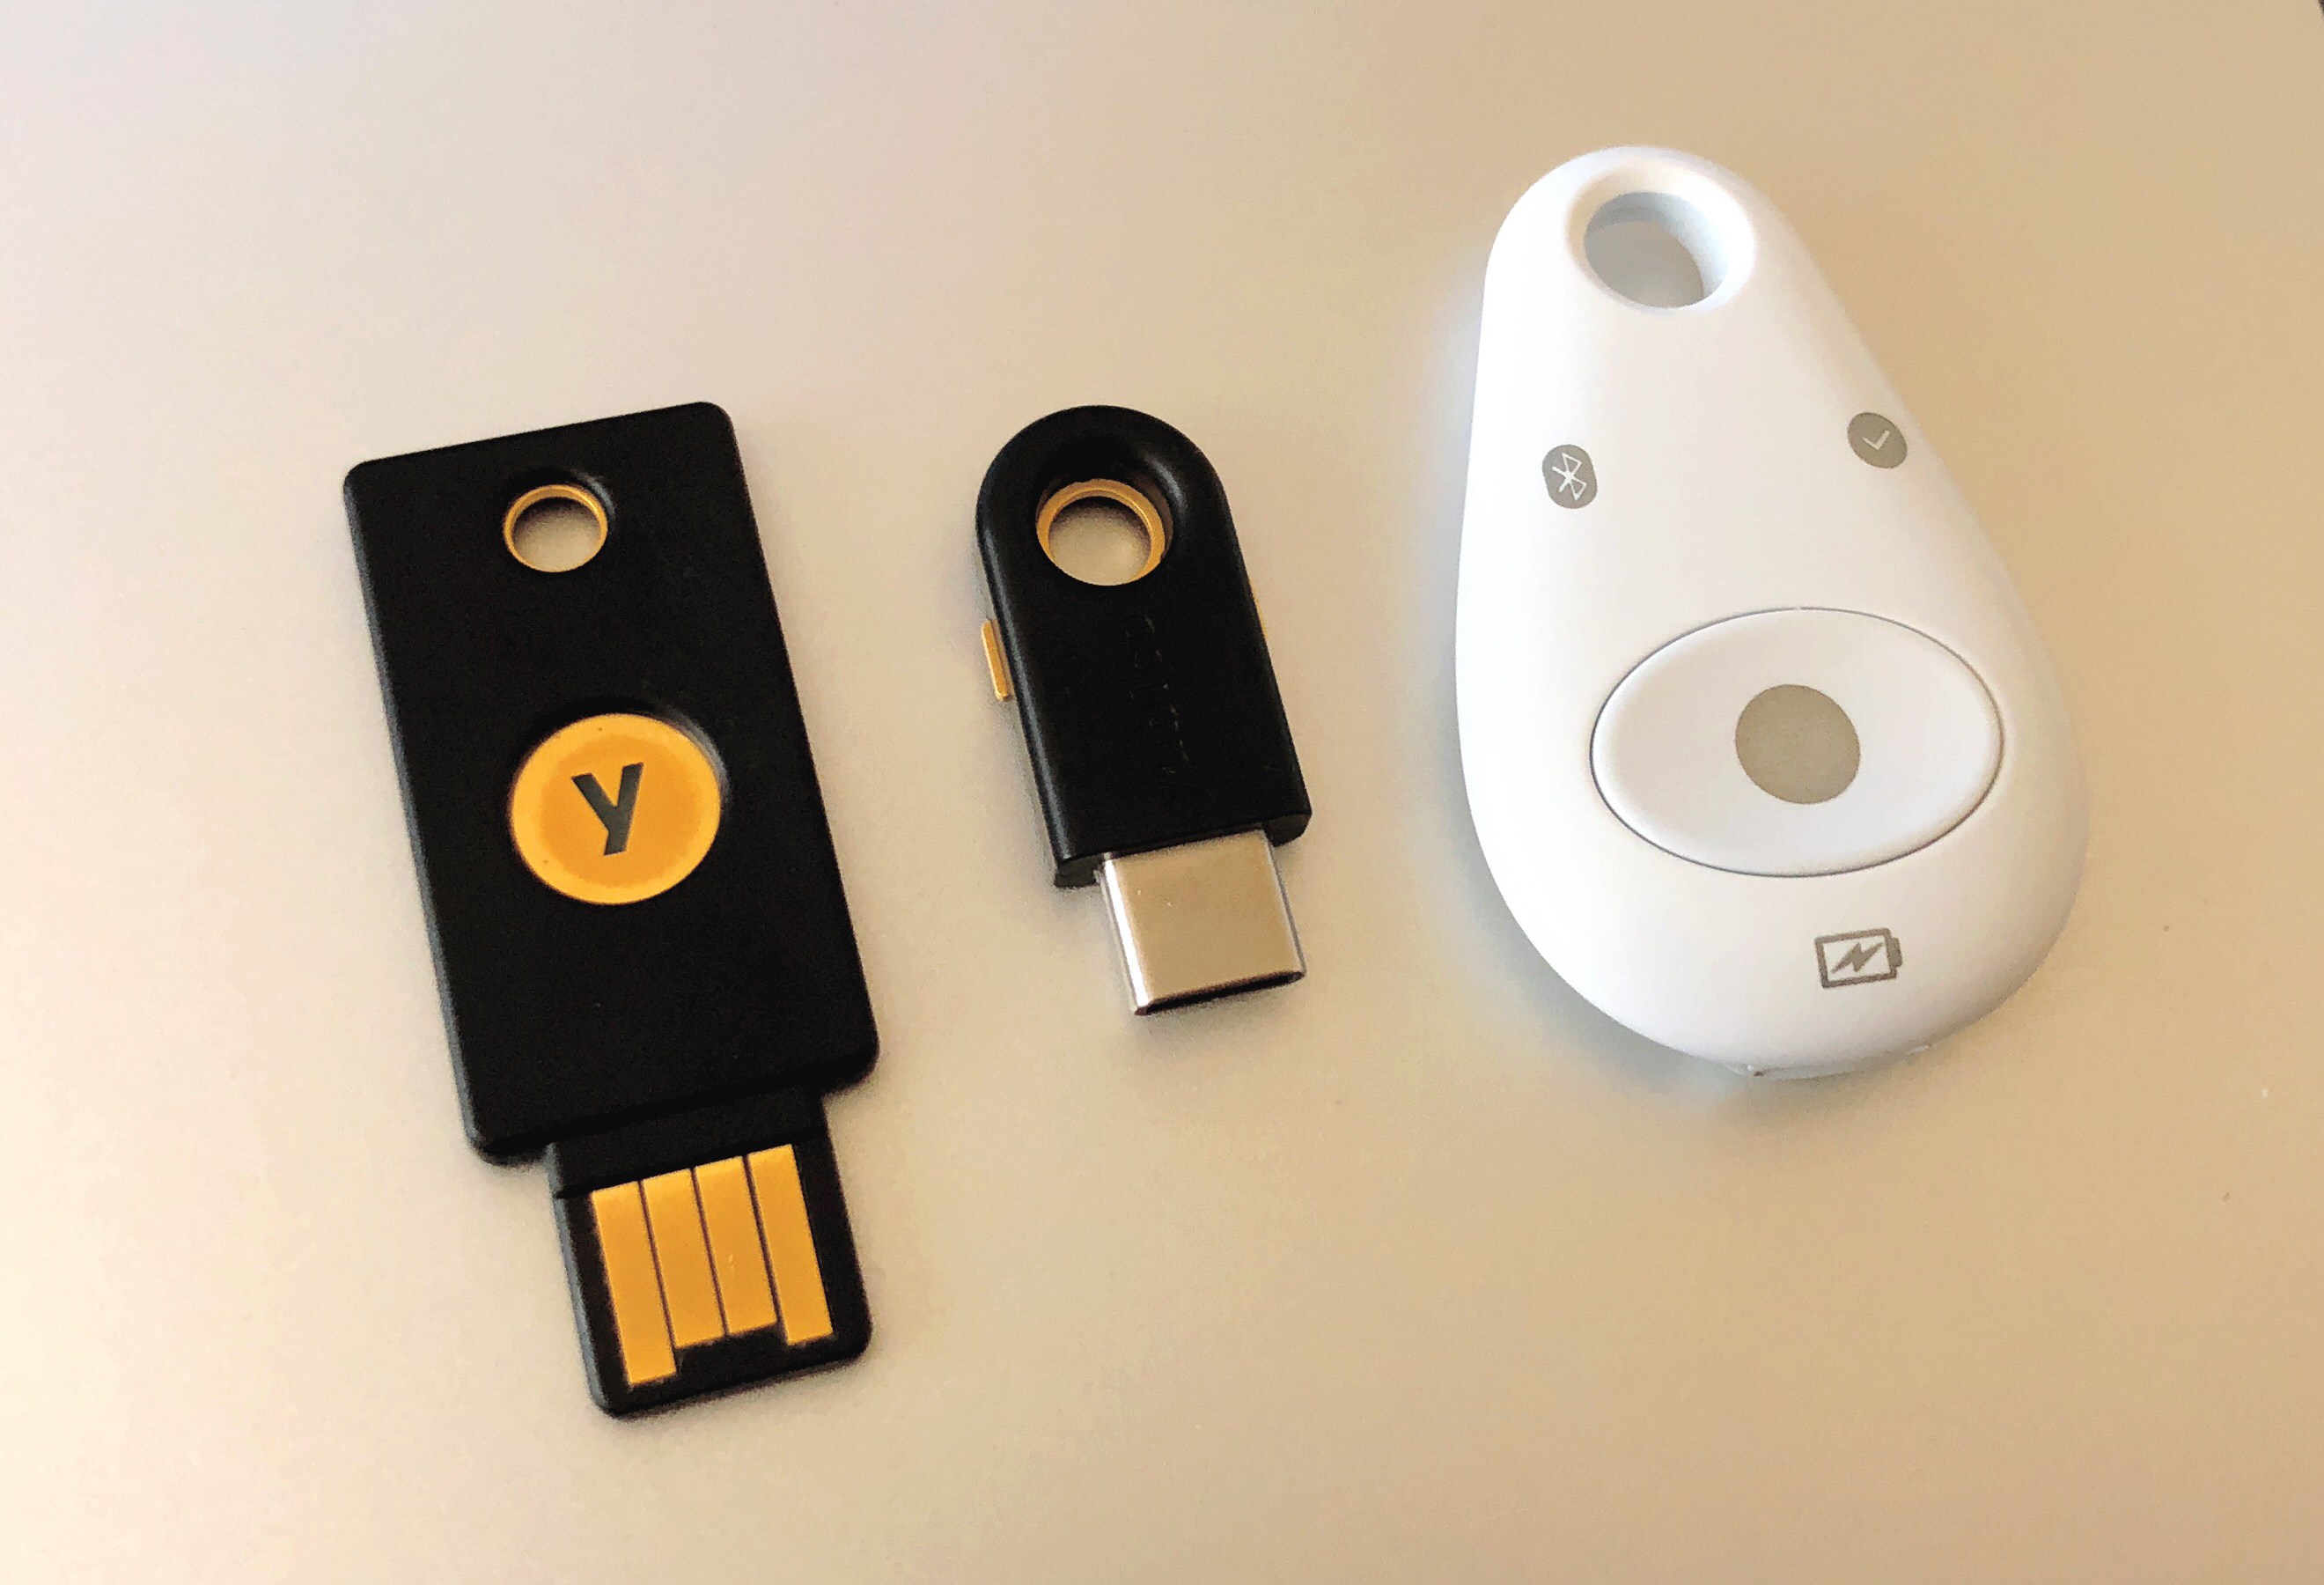
\includegraphics[width=0.8\linewidth]{04
      research/assets/hardware authentication.jpg}
    \caption{Proprietary Tokens}
    \parencite{img:authToken}
  \end{subfigure}

  \caption{Methods of accessing OTPs}
  \label{fig:otp}
\end{figure}

Generating OTPs first requires a \enquote{seed}: a secret
value unique to each user account.
It also requires a \enquote{moving factor}, which changes
with each request for an OTP.
With this data, an OTP can be generated using many
industry-standard algorithms like SHA-1
\parencite{whatIsOtp}.

With an HOTP (Hash-based Message Authentication Code
One-time Password), the moving factor is a counter
incremented every time an OPT is successfully verified.
Time-based OTPs (or TOTP) use a \enquote{timestep} as its
moving factor, which specifies a short window a time
relative to its time-of-generation in which the TOTP is
valid \parencite{whatIsOtp}.

\subsection{Biometrics}
\label{ss:biometrics}

Biometrics identify individuals using \enquote{distinctive
  physical characteristics}, categorised within the inherent
factor \parencite{surveyOnAuthFactors}.

\cite{evalOfAuthMethods,
  surveyOnAuthFactors} both identify these
standard characteristics:

\begin{itemize}
  \item Fingerprint
  \item Retina/Iris
  \item Speaker recognition
  \item Face recognition
  \item Hands
\end{itemize}

Although each characteristic requires specialist hardware
and/or software to read, some of the technologies have made
their way into modern smart devices.
Android and iOS both allow devices to be unlocked using a
fingerprint or facial recognition, with further support for
iris scanning on Android \parencite{androidBiometrics,
  touchId, faceId}.
An important characteristic of these authentication
mechanisms is the verification process is generalised to
anyone with biometric data registered to the device, as
opposed to a specific user/account \parencite[][Return
  value of getAuthenticationType()]
{androidBiometricAuthResult}.

\subsection{Conclusions}

Affirming the remarks in the
\hyperref[s:motivation]{project motivation}, the
conventional authentication factors explored above do not
account for conspiring users.
Passwords and OTPs can be easily shared, and biometrics
cannot identify a specific account associated to the
credential.

Furthermore, biometrics may constrain the potential
userbase: some people wear religious facial garments, some
people don't have fingerprints.

In a context with the potential for \gls{conspiring-users},
these methodologies alone are not adequate to authenticate
users, meaning \projectname{}'s identification process must
incorporate additional data to securely check-in employees.
